\subsection{Organisation du programme}
  Le projet contient :
  \begin{itemize}
    \item un \verb+README+, très complet avec entre autres les détails pour installer et configurer le programme ainsi que des explications et des exemples sur son utilisation ;
    \item un répertoire base, regroupant plusieurs librairies externes (sous
    licences compatibles GPLv2) ;
    \item un fichier de configuration ;
    \item \verb+queue.h/cc+, \verb+packet.h/cc+ et \verb+conntrack.h/cc+ qui réalisent l'interception des paquets envoyés à \verb+NFQUEUE+ (\verb+queue.cc+), leur
    interprétation (\verb+packet.cc+), et leur mise en relation avec un conntrack
    (\verb+conntrack.cc+) ;
    \item \verb+classifier.h/cc+ qui sert à classer les paquets ;
    \item un fichier de base permettant le lancement des threads, un autre parsant le fichier de configuration et initialisant le classifier.
  \end{itemize}

\subsection{Fonctionnement du logiciel}
  Afin de réaliser son objectif de classification des connexions http et ftp, notre extension NetFilter doit
  réaliser quatre étapes distinctes. Tout d'abord, il s'agit de regrouper les paquets appartenant à une même
  connexion; ensuite il faut déterminer si le contenu de la connexion correspond à un protocole supporté;
  puis la méthode et l'url utilisées par le client (par exemple {\tt GET /foo/bar.pdf}) doivent être extraites
  des paquets; enfin ces méthodes et cette url permettent de classifier la connexion, et de remonter l'information
  au noyau.
  
  \paragraph{Identification des paquets}
    Cette étape cruciale vise à rassembler les paquets appartenant à une même connexion, afin de pouvoir
    les traiter simultanément. Plus précisément, il s'agit d'identifier la connexion de chaque paquet,
    et d'agréger son contenu aux données déjà transférées.
    
    Cette étape est réalisée grâce à l'utilisation de \verb+libnetfilter_conntrack+, qui nous permet de
    maintenir en local une liste à jour des connexions connues par le noyau. L'identification d'un paquet
    à une connexion se fait en utilisant une clé unique, déterminée à partir des adresses et ports source
    et destination.

  \paragraph{Détermination du protocole}
    Grâce à l'identification des connexions, il a été possible de disposer, pour chacune de ces connexions,
    des buffers de données échangées entre les deux extrémités de la connexion.
    
    Cela permet alors, en utilisant des chaînes toujours présentes dans les protocoles analysés, de déterminer
    le type de la connexion. Par exemple, une requête HTTP peut se repérer à la chaîne ``{\tt <method> <url> http/<http-version>}''
    envoyée par le client, et à la réponse du serveur sous la forme ``{\tt <numerical-code> <message>}''.

  \paragraph{Extraction de l'URL}
    Dans le cas du protocole http, il s'agit d'une opération simple, qui utilise la première ligne du buffer egress (client
    vers serveur). Cette ligne permet d'extraire la méthode (GET, POST, ...), ainsi que l'url de la ressource demandée.
    
    Le protocole ftp est plus complexe à gérer, puisque d'une part la requête n'est pas disponible dès la première ligne d'un des buffers,
    et que d'autre part le client pourra légitimement accéder à plusieurs ressources, ce qui interdit une classification définitive.
    L'analyseur du protocole FTP détermine donc quel coté de la connexion est le client, puis, en analysant le buffer émis par le client,
    repère les requêtes, et met à jour l'information de classification au fur et à mesure de l'interprétation des nouveaux paquets.
    

  \begin{figure}[h]
    \centering
    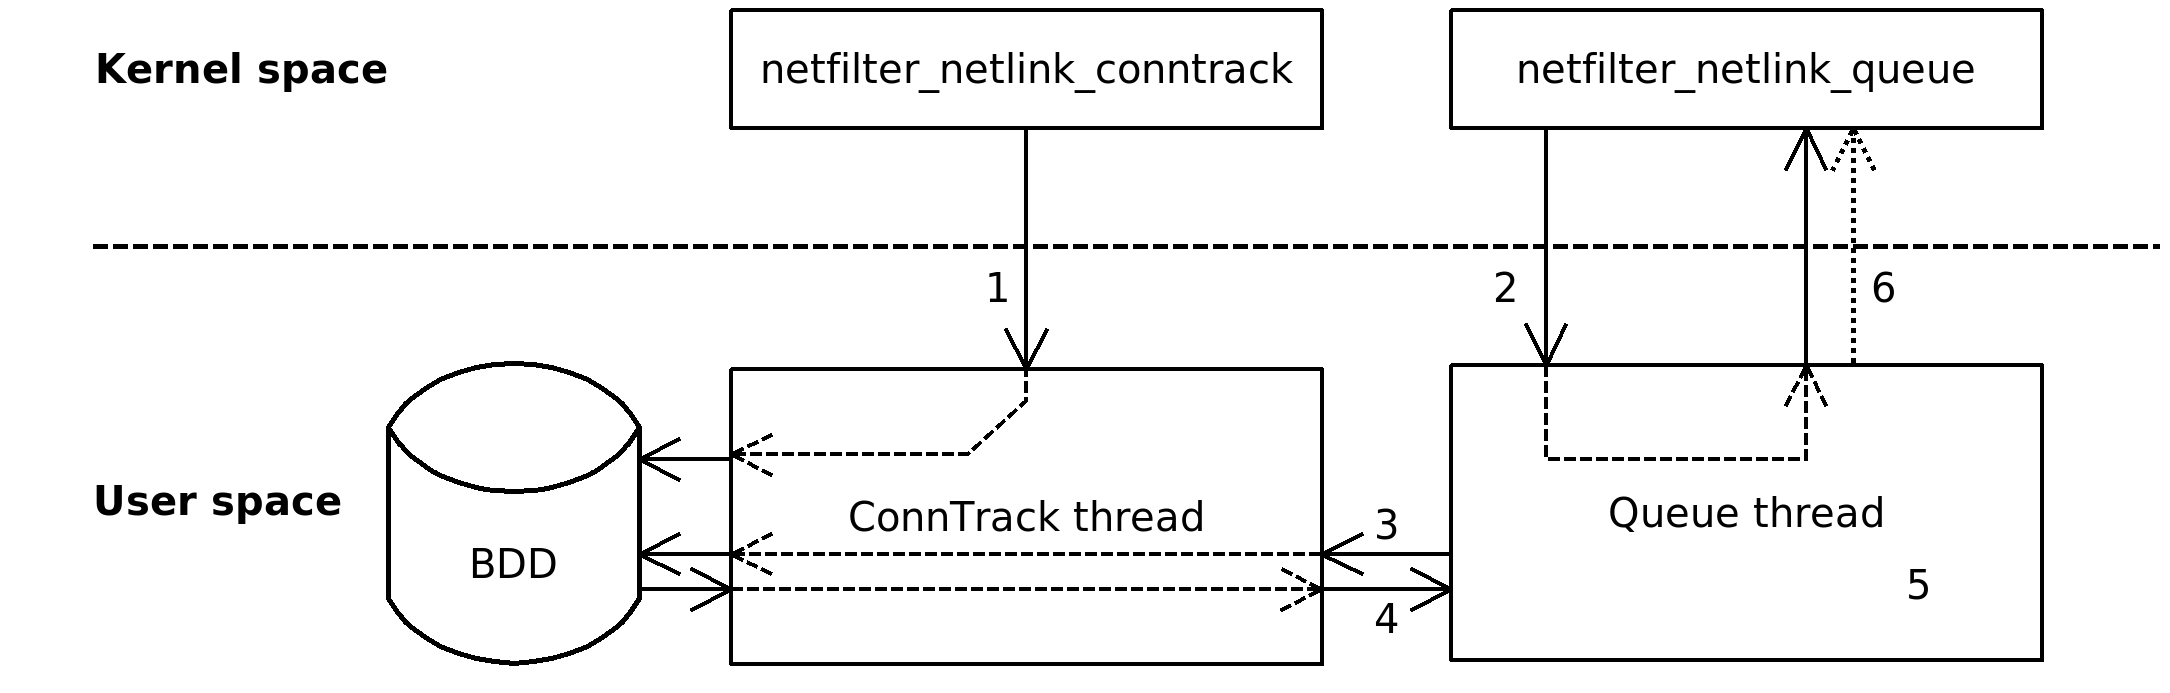
\includegraphics[width=\textwidth]{schema2.png}\\
    \title{Fonctionnement du module}
  \end{figure}

  \begin{footnotesize}
    \noindent Légende du schéma :
    \begin{enumerate}
    \item Maintien d'une copie locale de la base conntrack du noyau, grâce aux \og events \fg{} de la \verb+libnetfilter_conntrack+.
    \item Récupération des paquets envoyés sur \verb+NFQUEUE+ via la \verb+libnetfilter_queue+.
    \item Récupération, pour chaque paquet, des informations de conntrack existantes.
    \item Retour des informations de conntrack pour le paquet, en particulier le contenu des paquets précédents, pour permettre la classification.
    \item Classification basée exclusivement sur le contenu de la connexion.
    \item Réinjection du paquet et d'une \og mark \fg{} de classification dans la chaîne de filtrage netfilter du noyau.
    \end{enumerate}
  \end{footnotesize}

  \paragraph{Fonctionnement pratique}
    L'application a deux threads; le premier (cf. \verb+ConnTrack::Run()+) écoute sur un
    \verb+netfilter_netlink+, reçoit les mises à jour de la table conntrack du noyau, et
    maintient une copie locale.
    
    Le deuxième (cf. \verb+Queue::Run()+) intercepte les paquets arrivant sur une
    \verb+NFQUEUE+ (via \verb+iptables+), les parse, détermine l'entrée conntrack
    correspondante (en demandant à une table partagée avec l'autre
    thread), récupère l'objet \og Connection \fg{} correspondant, met à jour les
    deux buffers, puis appelle la méthode \verb+update+ du classifier ; enfin il
    accepte le paquet, en le marquant avec la mark déterminée par le
    classifier (ou une marque par défaut si pas de classifier).
    
    Le classifier regarde les buffers d'une connexion à chaque fois qu'ils sont mis à jour.
    Il prend ensuite une décision (NoMatch, NoMatchYet ou une vraie décision) ; le classifier retourne aussi un \og buffer hint \fg{} au conntrack : c'est à dire qu'il indique quelle
    partie du buffer lui est encore utile, pour que le conntrack puisse
    purger la partie inutile du buffer.

\subsection{Fiabilité et limitations}
  L'objectif d'un classifier tel que celui-ci est principalement de repérer, limiter, voire interdire certaines requêtes basées sur les protocoles ftp ou http.
  Il doit donc éviter au maximum d'être contournable par un client. Plusieurs points sont à évaluer: la bonne interprétation du protocole concerné, la résistance à la
  fragmentation de paquets, la résistance à l'inversion de paquets TCP, ou encore l'utilisation de version non-standard des protocoles (versions parfois supportées par
  les serveurs).
  
  Pour ce qui est de la partie protocolaire, notre \emph{urlfilter} gère correctement le protocole ftp, en particulier grâce à une grande tolérance dans la détection
  des requêtes; l'analyseur ftp gère également la présence de plusieurs requêtes successives lors d'une même session ftp.\\
  Notre analyseur http est par contre plus vulnérable; il ne gère en particulier pas les requêtes en \emph{Keep-Alive}, qui permettent de packer plusieurs requêtes dans une
  même connexion.
  
  Grâce aux buffers de connexions maintenus pour chaque connexion, l'application résiste nativement aux contournements par fragmentation des paquets, puisque ce n'est pas le
  contenu de chaque paquet qui est analysé, mais l'ensemble des données transférées. Par contre, les attaques par inversions de paquets ne sont pas gérées; le réordonnancement
  des paquets est en effet un problème non-trivial, qui semble dépasser le cadre du projet.
  
  Enfin, l'application est supposée résister aux attaques de types \emph{Denial of Service}, en limitant en particulier la quantité de données conservées pour une même connexion.
  En limitant à 64ko cette quantité, on évite qu'une connexion TCP spécialement conçue puisse entraîner la conservation d'un nombre non borné d'octets lors de la phase de
  détermination du protocole (en effet cette phase nécessite à minima la présence d'une ligne complète dans l'un des deux buffers).
